% Esqueleto do artigo v3 (PLANO_ARTIGO.md v3). Template: IEEE Conference (a confirmar com o professor).
% Compilar no Overleaf (classe IEEEtran). Números: SEMPRE pelas macros de numbers.tex (paper/make_numbers.py).
\documentclass[conference]{IEEEtran}
\usepackage[utf8]{inputenc}
\usepackage[T1]{fontenc}
\usepackage{amsmath,amssymb}
\usepackage{graphicx}
\usepackage{booktabs}
\usepackage{siunitx}
\usepackage[hidelinks]{hyperref}
% Gerado por paper/make_numbers.py a partir dos CSVs. NÃO EDITAR À MÃO.
\newcommand{\vOneSuccessPpoSTwo}{70.7}  % paper/tables/v1_rq1_taquari.csv: S2 ppo success
\newcommand{\vOneSuccessStraightSTwo}{70.0}  % paper/tables/v1_rq1_taquari.csv: S2 straight success
\newcommand{\vOneDiffSuccessSTwoLow}{-7.1}  % paper/tables/v1_rq1_taquari.csv: S2 ppo − straight, IC hierárquico
\newcommand{\vOneDiffSuccessSTwoHigh}{9.8}  % paper/tables/v1_rq1_taquari.csv: S2 ppo − straight, IC hierárquico
\newcommand{\vOneFalseLocPpoSTwo}{20.2}  % paper/tables/v1_rq1_taquari.csv: S2 ppo false loc
\newcommand{\vOneFalseLocStraightSTwo}{13.0}  % paper/tables/v1_rq1_taquari.csv: S2 straight false loc
\newcommand{\vOneDistSuccessPpoSTwo}{1.25}  % paper/tables/v1_rq1_taquari.csv: S2 ppo distance (successes), km
\newcommand{\vOneDistSuccessStraightSTwo}{1.89}  % paper/tables/v1_rq1_taquari.csv: S2 straight distance (successes), km
\newcommand{\vOneRhoColorMin}{-0.25}  % results_final/change_index/independent_covariate.csv: menor Spearman cor × sucesso
\newcommand{\vOneRhoColorMax}{-0.15}  % results_final/change_index/independent_covariate.csv: maior Spearman cor × sucesso
\newcommand{\vOneSuccessQOnePpo}{81.8}  % results_final/change_index/success_by_change_quintile.csv: taquari ppo Q1
\newcommand{\vOneSuccessQFivePpo}{63.2}  % results_final/change_index/success_by_change_quintile.csv: taquari ppo Q5
\newcommand{\vOneSuccessQOneStraight}{91.0}  % results_final/change_index/success_by_change_quintile.csv: taquari straight Q1
\newcommand{\vOneSuccessQFiveStraight}{53.8}  % results_final/change_index/success_by_change_quintile.csv: taquari straight Q5
\newcommand{\vOneMOneChangeDiff}{0.19}  % results_final/mechanism/m1.csv: taquari, mudança visitada, falsa − sucesso
\newcommand{\vOneMOneChangeDiffLow}{0.16}  % results_final/mechanism/m1.csv: IC
\newcommand{\vOneMOneChangeDiffHigh}{0.22}  % results_final/mechanism/m1.csv: IC
\newcommand{\vOneMOneVerdict}{não suportada}  % results_final/mechanism/m1.csv: veredito pelo critério F3
\newcommand{\moHFourVerdict}{não avaliável}  % results_mo_v1fix/verdicts_v2.json: H4
\newcommand{\moHSixVerdict}{não suportada}  % results_mo_v1fix/verdicts_v2.json: H6
\newcommand{\moEumSampled}{0.753}  % results_mo_v1fix/eum.csv
\newcommand{\moEumPocSampled}{0.764}  % results_mo_v1fix/eum.csv


\begin{document}

% Título: escolher no domingo, 22/11, com os resultados (PLANO_ARTIGO.md §1).
\title{Change-Aware Active Localization for GNSS-Denied UAVs over Outdated Post-Flood Maps}
\author{\IEEEauthorblockN{Autores a definir}\IEEEauthorblockA{UFRGS}}
\maketitle

\begin{abstract}
% Escrever na segunda, 23/11 (Vitor), depois do congelamento: pergunta, abordagem (PPO sobre a crença, à la ANL),
% dados reais de enchente, 3 achados com números (macros), conclusão. 150–250 palavras, sem citações.
\end{abstract}
\begin{IEEEkeywords}
Active localization, reinforcement learning, belief space, UAV, visual geo-localization, outdated maps, disaster response.
\end{IEEEkeywords}

\section{Introduction}
\label{sec:intro}
% ~0,7 pág. (PLANO_ARTIGO.md v4 §4). Drone sem GNSS e mapa anterior ao desastre; localização ativa como POMDP;
% pergunta "quando aprender a agir compensa?". Contribuições: (i) adaptação do ANL com PPO a imagens reais antes/depois
% de enchente em 4 locais; (ii) comparação pareada com heurísticas fortes (eficiência × risco); (iii) resultado
% negativo do MOPPO, com diagnóstico; (iv) evidência de que o valor da política depende da ambiguidade perceptual
% (v3 + experimento E, exploratório). Relação explícita com o ANL \cite{chaplot2018anl} e com o AMOR \cite{alegre2025amor}.

\section{Related Work}
% Rascunho da IA-2 (quinta). A: localização ativa; B: localização visual absoluta de UAV e reconhecimento de lugar;
% C: mapas desatualizados e mapeamento de desastres; D: avaliação confiável em RL (rliable); posicionamento.

\section{Preliminary Study: Why Active Localization Fails on Outdated Maps}
\label{sec:preliminary}
% ~0,8 pág. Números só por macro (numbers.tex). Fig.~\ref{fig:motivation}.
% (1) Em S2, a PPO não se distingue da reta em sucesso: \vOneSuccessPpoSTwo\% × \vOneSuccessStraightSTwo\%,
%     IC hierárquico da diferença [\vOneDiffSuccessSTwoLow; \vOneDiffSuccessSTwoHigh] p.p.; ~2/3 da distância nos
%     sucessos (\vOneDistSuccessPpoSTwo × \vOneDistSuccessStraightSTwo km); mais localizações falsas
%     (\vOneFalseLocPpoSTwo\% × \vOneFalseLocStraightSTwo\%).
% (2) O sucesso de todos os métodos cai com o índice de mudança (F1); a covariável de cor, independente do
%     descritor, aponta na mesma direção (Spearman de \vOneRhoColorMin a \vOneRhoColorMax, F2).
% (3) Mecanismo M1 (\vOneMOneVerdict): localizações falsas visitam células mais mudadas (+\vOneMOneChangeDiff,
%     IC [\vOneMOneChangeDiffLow; \vOneMOneChangeDiffHigh]), mas não mais distintivas nem mais que as da reta.
%     ATENÇÃO: isso muda a tese do PLANO_ARTIGO.md §1 (ver STATUS_V3.md).
\begin{figure}[t]
\centering
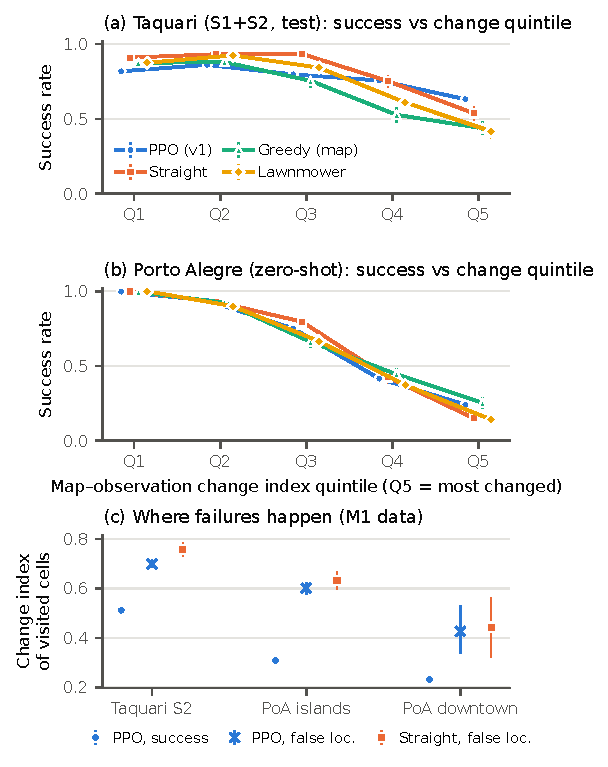
\includegraphics[width=\columnwidth]{figures/fig2_v1_motivation.pdf}
\caption{Preliminary study (v1). (a,b) Success rate by map--observation change-index quintile. (c) Change index of the cells visited in successful and false-localization episodes.}
\label{fig:motivation}
\end{figure}

\section{Problem Formulation}
% ~0,5 pág. POMDP (posição contínua, altitude, 10 ações, 80 passos, custo em tempo de voo); footprint 2h tan(FOV/2);
% deriva; atualização bayesiana; verossimilhança temperada; verossimilhança CA (mistura com rho = alpha m); entropia;
% sucesso, localização falsa e timeout (a parada usa só a crença).

\section{Method}
% ~1,0 pág. A: descritor (DINOv2 + GeM + PCA; ajuste fino contrastivo só na faixa de treino);
% B: filtro ciente da mudança (prior EMSR720 com fontes até 06/05/2024; EMSN194 em POA, rotulado "otimista");
% C: política (PPO à la ANL + canal m; variante com altitude); D: ambiente em lote e paridade (G2).
% Fig. 1: visão geral (a criar).

\section{Experimental Setup}
% ~0,6 pág. Tabela I (áreas, datas, prior, dobras); validação espacial em 3 faixas; zero-shot;
% métodos e ablações; estatística (10 seeds, rliable, bootstrap hierárquico, Holm); hardware e tempo de GPU.

\section{Results}
% ~1,9 pág. A: percepção (H1); B: principal (H3, Tabela II, Fig. 3); C: filtro CA (H2, Fig. 4);
% D: altitude (H4, Fig. 5); E: transferência (H5) e validação espacial; F: ablações (Tabela III).
% Uma frase de veredito por hipótese, no formato do critério (DECISIONS_V3.md §2).

\section{Discussion}
% ~0,6 pág. O que o prior resolve e o que não; quando a escolha ativa paga a pena; MO em 1 frase (apêndice);
% limitações; ameaças à validade (dependência espacial, padronização transdutiva no estudo v1, sobreposição das
% regiões, desalinhamento local, índice dependente do descritor, alterações de critério e de protocolo).

\section{Conclusion}
% ~0,2 pág. Responder às 3 perguntas; trabalhos futuros.


\bibliographystyle{IEEEtran}
\bibliography{refs}

\appendix
\section{Preliminary-study verdicts and multi-objective extension}
% Vereditos do estudo v1 e tabela de alterações de critério e de protocolo.
% MO: errata; H4 \moHFourVerdict; H6 \moHSixVerdict; EUM amostrado \moEumSampled{} (MO) × \moEumPocSampled{} (PoC).


\end{document}
